\section{Experiment}

\subsection{Measurement of voltage source parameters}

The voltage source parameters were measured twice during this laboratory. 

\subsubsection*{1st experiment}

In the first experiment we connected an oscilloscope to the circuit (Fig.~\ref{fig:voltage_osc}). Measurements were taken for varying load resistances and stopped once the $\frac{V}{V_o}$ ratio fell below $0.95$. Current was calculated using the Ohm's Law and peak-to-peak voltage value was read from the oscilloscope. All measurements are shown in Table~\ref{tab:voltage_osc}. Figure~\ref{fig:volt-curr_osc} shows the voltage-current characteristics of a voltage source. 

\begin{figure}[H]
	\centering
	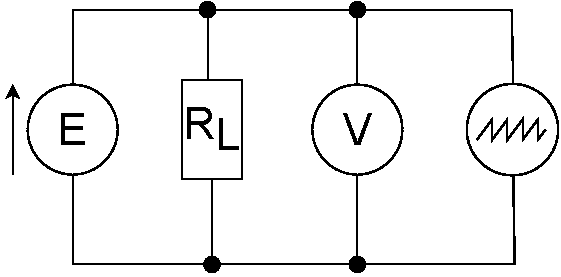
\includegraphics[width=6cm]{schematics/1.pdf}
	\caption{Voltage source parameters measurement ($R_L$ -- load resistance).}
	\label{fig:voltage_osc}
\end{figure}

\begin{table}[H]
	\centering
	\begin{tabular}{ c | c | c | c | c}
		$R_L [\unit{\ohm}]$ & $V [\unit{\volt}]$ & $\frac{V}{V_o}$ & $V_{p-p}[\unit{\milli\volt}]$ & $I [\unit{\milli\ampere}]$ \\
		\hline
		$10000$ & $5.31131$ & $0.99909$ & $19.6$ & $0.53113$ \\
		$9000$ & $5.31236$ & $0.99929$ & $18$ & $0.59026$ \\
		$8000$ & $5.31491$ & $0.99977$ & $18.4$ & $0.66436$ \\
		$7000$ & $5.315501$ & $0.99988$ & $19.2$ & $0.75936$ \\
		$6000$ & $5.31475$ & $0.99974$ & $18.8$ & $0.88579$ \\
		$5000$ & $5.3145$ & $0.99969$ & $18$ & $1.06290$ \\
		$4000$ & $5.31252$ & $0.99932$ & $16.4$ & $1.32813$ \\
		$3000$ & \textcolor{BrickRed}{$5.31252$} & $0.99932$ & $20.4$ & \textcolor{BrickRed}{$1.77084$} \\
		$2000$ & \textcolor{ForestGreen}{$5.30828$} & $0.99852$ & $18.8$ & \textcolor{ForestGreen}{$2.65414$} \\
		$1000$ & \textcolor{BrickRed}{$5.31172$} & $0.99917$ & $18$ & \textcolor{BrickRed}{$5.31172$} \\
		$900$ & $5.31169$ & $0.99916$ & $19.6$ & $5.90188$ \\
		$800$ & \textcolor{ForestGreen}{$5.31252$} & $0.99932$ & $17.2$ & \textcolor{ForestGreen}{$6.64065$} \\
		$700$ & \textcolor{blue}{$5.31295$} & $0.99940$ & $19.6$ & \textcolor{blue}{$7.58993$} \\
		$600$ & \textcolor{blue}{$5.31366$} & $0.99953$ & $15.2$ & \textcolor{blue}{$8.85610$} \\
		$500$ & $5.31247$ & $0.99931$ & $17.6$ & $10.62494$ \\
		$400$ & $5.14929$ & $0.96861$ & $50.4$ & $12.87323$ \\
		$300$ & $4.92745$ & $0.92688$ & $100$ & $16.42483$ \\ 
	\end{tabular}
	\caption{Voltage source parameters measurements for $V_o=\SI{5.31615}{\volt}$ ($R_L$ -- load resistance, $V_o$ -- measured voltage for $R_L = \SI{0}{\ohm}$, $V_{p-p}$ -- peak-to-peak voltage).}
	\label{tab:voltage_osc}
\end{table}

\begin{figure}[H]
	\centering
	\begin{subfigure}{.5\textwidth}
		\centering
		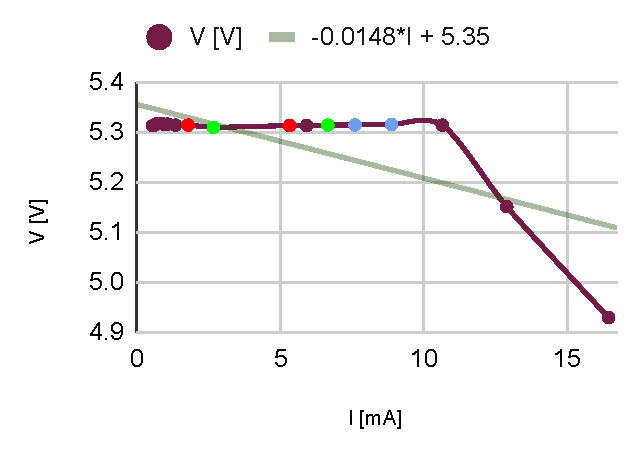
\includegraphics[width=.99\linewidth]{schematics/chart1.pdf}
	\end{subfigure}%
	\begin{subfigure}{.5\textwidth}
		\centering
		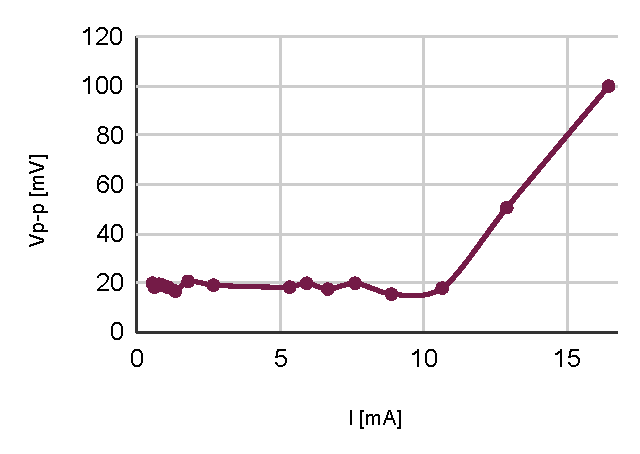
\includegraphics[width=.99\linewidth]{schematics/chart2.pdf}
	\end{subfigure}
	\caption{Voltage-current characteristics of a voltage source.}
	\label{fig:volt-curr_osc}
\end{figure}

Using the $V=f(I)$ graph and the trend line defined by the equation $V =  - I\cdot R_{int} + E$, the following values can be obtained:
\begin{itemize}
	\item $R_{int}$ (internal resistance defined as the slope of the trend line): $\SI{14.8}{\ohm}$;
	\item $E$ (electromotive force): $\SI{5.35}{\volt}$;
	\item $I_{max}$ (maximal current for which the power supply works like an ideal one): $\approx \SI{10}{\milli\ampere}$.
\end{itemize}

Table~\ref{tab:voltage_2point} shows the parameters calculated using the two-point method.

\begin{table}[H]
	\centering
	\begin{tabular}{  c | c | c | c | c | c | c}
		Points & $V_1 [\unit{\volt}]$ & $I_1 [\unit{\milli\ampere}]$ & $V_2 [\unit{\volt}]$ & $I_2 [\unit{\milli\ampere}]$ & $R_{int} [\unit{\ohm}]$ & $E [\unit{\volt}]$ \\
		\hline
		\textcolor{BrickRed}{Red} & $5.31252$ & $1.77084$ & $5.31172$ & $5.31172$ & $0.22593$ & $5.31292$ \\
		\textcolor{ForestGreen}{Green} & $5.30828$ & $2.65414$ & $5.31252$ & $6.64065$ & $-1.06359$ & $5.30546$ \\
		\textcolor{blue}{Blue} & $5.31295$ & $7.58993$ & $5.31366$ & $8.85610$ & $-0.56075$ & $5.30869$ \\
	\end{tabular}
	\caption{Voltage source parameters.}
	\label{tab:voltage_2point}
\end{table}

$E$ and $R_{int}$ were obtained using the formulas shown in Equation~\ref{eq:dupa}.

\begin{equation}
	\begin{cases}
			E = I_1\cdot R_{int} + V_1\\
			E = I_2\cdot R_{int} + V_2
	\end{cases}
	\begin{cases}
		R_{int} = \frac{V_1-V_2}{I_2-I_1}\\
		E = I\cdot R_{int} + V
	\end{cases}
	\label{eq:dupa}
\end{equation}


\subsubsection*{2nd experiment}

In the second experiment we disconnected the oscilloscope and added an ammeter to the circuit (Fig.~\ref{fig:voltage}). Measurements were made for varying load resistance values and stopped once the $\frac{V}{V_o}$ ratio fell below $0.95$. All measurements are shown in Table~\ref{tab:2}. Figure~\ref{fig:2} shows the voltage-current characteristics of a voltage source. 

\begin{figure}[H]
	\centering
	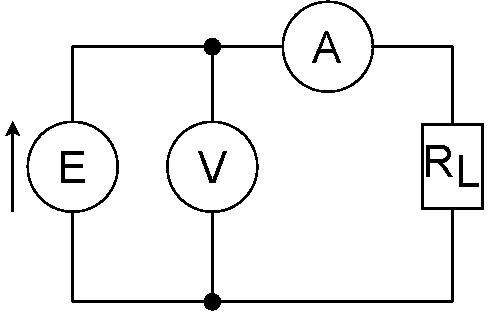
\includegraphics[width=6cm]{schematics/2.pdf}
	\caption{Voltage source parameters measurement ($R_L$ -- load resistance).}
	\label{fig:voltage}
\end{figure}

\begin{table}[H]
	\begin{subtable}[c]{0.5\textwidth}
		\centering
			\begin{tabular}{ c | c | c | c}
			$R_L [\unit{\ohm}]$ & $V [\unit{\volt}]$ & $\frac{V}{V_o}$ & $I [\unit{\milli\ampere}]$ \\
			\hline
			$10000$ & $5.318$ & $0.99906$ & $0.53137$ \\
			$9000$ & $5.319$ & $0.99925$ & $0.59025$ \\
			$8000$ & $5.319$ & $0.99925$ & $0.66377$ \\
			$7000$ & $5.317$ & $0.99887$ & $0.75821$ \\
			$6000$ & $5.317$ & $0.99887$ & $0.88412$ \\
			$5000$ & $5.315$ & $0.99850$ & $1.06036$ \\
			$4000$ & $5.312$ & $0.99793$ & $1.3242$ \\
			$3000$ & \textcolor{BrickRed}{$5.306$} & $0.99681$ & 	\textcolor{BrickRed}{$1.76291$} \\
			$2000$ &	\textcolor{BrickRed}{$5.298$} & $0.99530$ & 	\textcolor{BrickRed}{$2.58513$} \\
			$1000$ & 	\textcolor{ForestGreen}{$5.271$} & $0.99023$ & 	\textcolor{ForestGreen}{$4.95231$} \\
			$900$ & 	\textcolor{ForestGreen}{$5.265$} & $0.98910$ & 	\textcolor{ForestGreen}{$5.53997$} \\
			$800$ & 	\textcolor{blue}{$5.255$} & $0.98723$ & \textcolor{blue}{$6.34545$} \\
			$700$ & \textcolor{blue}{$5.243$} & $0.98497$ & \textcolor{blue}{$7.21971$} \\
			$600$ & $5.228$ & $0.98215$ & $8.36787$ \\
			$500$ & $5.200$ & $0.97689$ & $9.96317$ \\
			$400$ & $5.144$ & $0.96637$ & $12.1929$ \\
			$300$ & $4.887$ & $0.91809$ & $15.2643$ \\
		\end{tabular}
		\subcaption{1st voltage source: $V_o=\SI{5.323}{\volt}$}
	\end{subtable}
	\begin{subtable}[c]{0.5\textwidth}
		\centering
			\begin{tabular}{ c | c | c | c}
			$R_L [\unit{\ohm}]$ & $V [\unit{\volt}]$ & $\frac{V}{V_o}$ & $I [\unit{\milli\ampere}]$ \\
			\hline
			$10000$ & $13.86$ & $0.99856$ & $1.38284$ \\
			$9000$ & $13.86$ & $0.99856$ & $1.51444$ \\
			$8000$ & $13.86$ & $0.99856$ & $1.70754$ \\
			$7000$ & $13.86$ & $0.99856$ & $1.95128$ \\
			$6000$ & $13.85$ & $0.99784$ & $2.28445$ \\
			$5000$ & $13.85$ & $0.99784$ & $2.76018$ \\
			$4000$ & 	\textcolor{BrickRed}{$13.85$} & $0.99784$ & 	\textcolor{BrickRed}{$3.44949$} \\
			$3000$ & $13.85$ & $0.99784$ & $4.59595$ \\
			$2000$ & 	\textcolor{ForestGreen}{$13.85$} & $0.99784$ & 	\textcolor{ForestGreen}{$6.87844$}\\
			$1000$ & 	\textcolor{BrickRed}{$13.84$} & $0.99712$ &	\textcolor{BrickRed}{$13.6041$} \\
			$900$ & 	\textcolor{ForestGreen}{$13.83$} & $0.9940$ & 	\textcolor{ForestGreen}{$15.0913$} \\
			$800$ & $13.83$ & $0.99640$ & $16.8573$ \\
			$700$ &	\textcolor{blue}{ $13.82$} & $0.99568$ & \textcolor{blue}{ $18.3644$ }\\
			$600$ & \textcolor{blue}{ $13.81$} & $0.99496$ & \textcolor{blue}{ $22.5856$} \\
			$500$ & $13.8$ & $0.99424$ & $27.0082$ \\
			$400$ & $13.79$ & $0.99352$ & $33.6526$ \\
			$300$ & $13.78$ & $0.99280$ & $44.6311$ \\
			$200$ & $13.68$ & $0.98559$ & $65.1863$ \\
			$100$ & $13.66$ & $0.98415$ & $132.8120$ \\
			$50$ & $13.37$ & $0.96326$ & $251.9140$ \\
		\end{tabular}
		\subcaption{2nd voltage source: $V_o=\SI{13.88}{\volt}$}
	\end{subtable}
	\caption{Voltage source parameters measurements ($R_L$ -- load resistance, $V_o$ -- measured voltage for $R_L = \SI{0}{\ohm}$)}
	\label{tab:2}
\end{table}

\begin{figure}[H]
	\centering
	\begin{subfigure}{.5\textwidth}
		\centering
		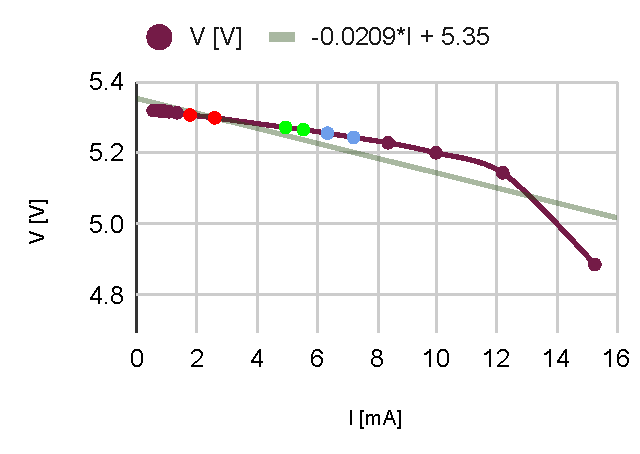
\includegraphics[width=.99\linewidth]{schematics/chart3.pdf}
		\caption{1st voltage source}
	\end{subfigure}%
	\begin{subfigure}{.5\textwidth}
		\centering
		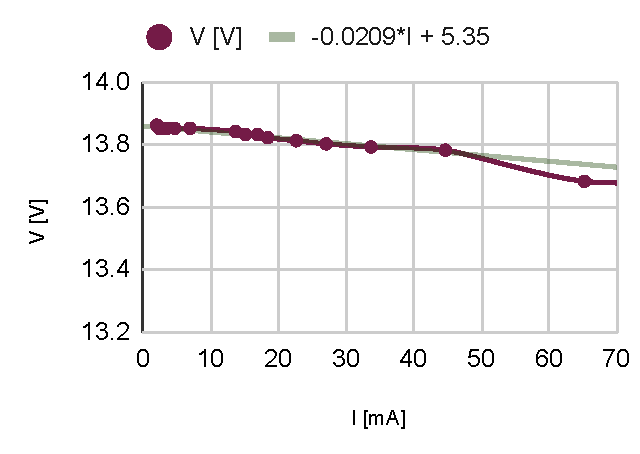
\includegraphics[width=.99\linewidth]{schematics/chart4.pdf}
		\caption{2nd voltage source}
	\end{subfigure}
	\caption{Voltage-current characteristics of a voltage source.}
	\label{fig:2}
\end{figure}

Similarly as in the first experiment, the parameters can be obtained using the graph and the trend line. For the first voltage source we get:
\begin{itemize}
	\item $R_{int} = \SI{20.9}{\ohm}$;
	\item $E=\SI{5.35}{\volt}$;
	\item $I_{max}\approx \SI{10}{\milli\ampere}$.
\end{itemize}

And for the second voltage source:
\begin{itemize}
	\item $R_{int} =  \SI{1.88}{\ohm}$;
	\item $E=\SI{13.9}{\volt}$;
	\item $I_{max}\approx \SI{30}{\milli\ampere} $.
\end{itemize}

Tables~\ref{tab:1},~\ref{tab:22} show the parameters calculated using the two-point method.

\begin{table}[H]
	\centering
	\begin{tabular}{  c | c | c | c | c | c | c}
		Points & $V_1 [\unit{\volt}]$ & $I_1 [\unit{\milli\ampere}]$ & $V_2 [\unit{\volt}]$ & $I_2 [\unit{\milli\ampere}]$ & $R_{int} [\unit{\ohm}]$ & $E [\unit{\volt}]$ \\
		\hline
		\textcolor{BrickRed}{Red} & $5.306$ & $1.76291$ & $5.298$ & $2.58513$ & $9.72976$ & $5.32315$ \\
		\textcolor{ForestGreen}{Green} & $5.271$ & $4.95231$ & $5.265$ & $5.53997$ & $10.20999$ & $5.32156$ \\
		\textcolor{blue}{Blue} & $5.255$ & $6.34545$ & $5.243$ & $7.21971$ & $13.72589$ & $5.34210$ \\
		
	\end{tabular}
	\caption{1st voltage source parameters.}
	\label{tab:1}
\end{table}

\begin{table}[H]
	\centering
	\begin{tabular}{  c | c | c | c | c | c | c}
		Points & $V_1 [\unit{\volt}]$ & $I_1 [\unit{\milli\ampere}]$ & $V_2 [\unit{\volt}]$ & $I_2 [\unit{\milli\ampere}]$ & $R_{int} [\unit{\ohm}]$ & $E [\unit{\volt}]$ \\
		\hline
			\textcolor{BrickRed}{Red} & $13.85$ & $3.44949$ & $13.84$ & $13.6041$ & $0.98477$ & $13.85340$ \\
		\textcolor{ForestGreen}{Green} & $13.85$ & $6.87844$ & $13.83$ & $15.0913$ & $2.43521$ & $13.86675$ \\
		\textcolor{blue}{Blue}  & $13.82$ & $18.3644$ & $13.81$ & $22.5856$ & $2.36899$ & $13.86351$ \\
	\end{tabular}
	\caption{2nd voltage source parameters.}
	\label{tab:22}
\end{table}

$E$ and $R_{int}$ were obtained using the formulas shown in Equation~\ref{eq:dupa}.

\subsection{Measurement of current source parameters}

To measure current source parameters we added a \SI{10}{\ohm} standard resistor to the circuit (Fig.\ref{fig:current}). Measurements were taken for varying load resistances and stopped once the $\frac{V}{V_o}$ ratio fell below 0.99. All measurements are shown in Table~\ref{tab:current}. Figure~\ref{fig:currcurr} shows the current-voltage characteristics of a current source. 

\begin{figure}[H]
	\centering
	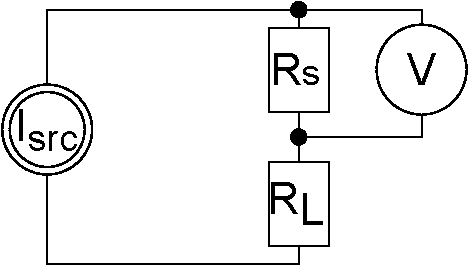
\includegraphics[width=6cm]{schematics/3.pdf}
	\caption{Current source parameters measurement ($R_L$ -- load resistance, $R_s$ -- standard resistor).}
	\label{fig:current}
\end{figure}

\begin{table}[H]
	\centering
	\begin{tabular}{ c | c | c | c | c}
		$R_L [\unit{\ohm}]$ & $V_v[\unit{\milli\volt}]$ & $\frac{V_v}{V_o}$ & $I [\unit{\milli\ampere}]$ & $V [\unit{\volt}]$ \\
		\hline
		$0$ & $19.3363$ & $1.00000$ & $1.93363$ & $0.0193363$ \\
		$10$ & $19.4437$ & $1.00555$ & $1.94437$ & $0.0388874$ \\
		$20$ & $19.4527$ & $1.00602$ & $1.94527$ & $0.0583581$ \\
		$30$ & $19.4569$ & $1.00624$ & $1.94569$ & $0.0778276$ \\
		$40$ & $19.4585$ & $1.00632$ & $1.94585$ & $0.0972925$ \\
		$50$ & $19.4607$ & $1.00643$ & $1.94607$ & $0.1167642$ \\
		$60$ & $19.4627$ & $1.00654$ & $1.94627$ & $0.1362389$ \\
		$70$ & $19.4633$ & $1.00657$ & $1.94633$ & $0.1557064$ \\
		$80$ & $19.4639$ & $1.00660$ & $1.94639$ & $0.1751751$ \\
		$90$ & $19.464$ & $1.00660$ & $1.9464$ & $0.19464$ \\
		$100$ & $19.4647$ & $1.00664$ & \textcolor{BrickRed}{$1.94647$} & \textcolor{BrickRed}{$0.2141117$} \\
		$200$ & $19.4199$ & $1.00432$ & \textcolor{BrickRed}{$1.94199$} & \textcolor{BrickRed}{$0.4078179$} \\
		$500$ & $19.4347$ & $1.00509$ & \textcolor{blue}{$1.94347$} & \textcolor{blue}{$0.9911697$} \\
		$1000$ & $19.4332$ & $1.00501$ & \textcolor{ForestGreen}{$1.94332$} & \textcolor{ForestGreen}{$1.9627532$} \\
		$2000$ & $19.4207$ & $1.00436$ & \textcolor{ForestGreen}{$1.94207$} & \textcolor{ForestGreen}{$3.9035607$} \\
		$5000$ & $19.3332$ & $0.99984$ & \textcolor{blue}{$1.93332$} & \textcolor{blue}{$9.6859332$} \\
		$6000$ & $16.8815$ & $0.87305$ & $1.68815$ & $10.1457815$ \\
	\end{tabular}
	\caption {Current source parameters measurements for $V_o = \SI{19.3363}{\milli\volt}$ ($R_L$ -- load resistance,  $V_v$ -- voltage drop on the standard resistor, $V_o$ -- measured voltage for $R_L = \SI{0}{\ohm}$).}
	\label{tab:current}
\end{table}

\begin{figure}[H]
	\centering
	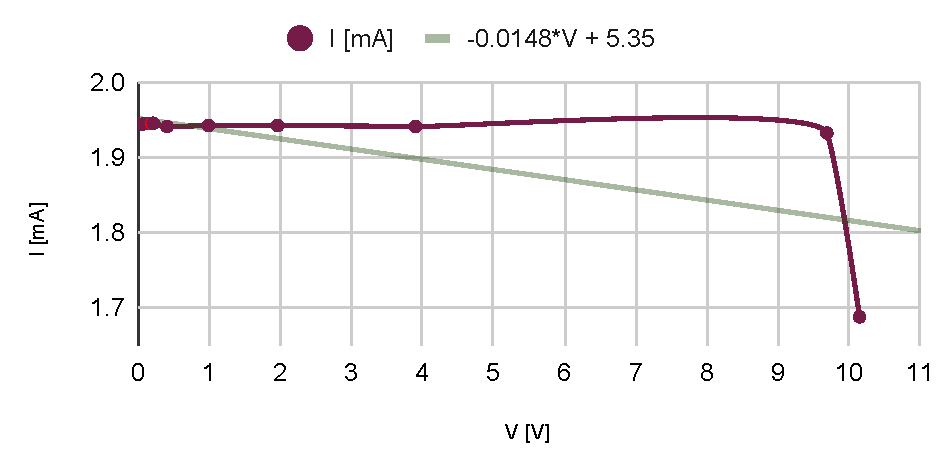
\includegraphics[width=10cm]{schematics/chart5.pdf}
	\caption{Current-voltage characteristics of a current source. }
	\label{fig:currcurr}
\end{figure}


Looking at the graph, we estimated the maximal voltage to be about \SI{9}{\volt}. Table~\ref{tab:kupa} shows the parameters calculated using the two-point method.

\begin{table}[H]
	\centering
	\begin{tabular}{ c | c | c | c | c | c | c}
		Points & $V_1 [\unit{\volt}]$ & $I_1 [\unit{\milli\ampere}]$ & $V_2 [\unit{\volt}]$ & $I_2 [\unit{\milli\ampere}]$ & $R_{int} [\unit{\ohm}]$ & $I_{src} [\unit{\milli\ampere}]$ \\
		\hline
		\textcolor{BrickRed}{Red} & $0.21411$ & $1.94647$ & $0.40782$ & $1.94199$ & $43238.83929$ & $1.94647$ \\
		\textcolor{ForestGreen}{Green} & $1.96275$ & $1.94332$ & $3.90356$ & $1.94207$ & $1552648$ & $1.94332$ \\
		\textcolor{blue}{Blue} & $0.99117$ & $1.94347$ & $9.68593$ & $1.93332$ & $856626.60099$ & $1.94347$ \\
	\end{tabular}
	\caption{Current source parameters ($R_{int}$-- internal resistance of the current source, $I_{src}$--nominal value).}
	\label{tab:kupa}
\end{table}

Current $I $ and voltage $V$ were obtained using the following formulas:
 
 
 \begin{equation}
 	\begin{cases}
 		I = \frac{V_v}{R_s}\\
 		V = I\cdot(R_L + R_s)
 	\end{cases}
 \end{equation}
 
And $R_{int}$ and $I_{src}$ were obtained using these:

\begin{equation}
	\begin{cases}
		I_1 =I_{src}- \frac{V_1}{R{int}}\\
		I_2 =I_{src}- \frac{V_2}{R{int}}
	\end{cases}
	\begin{cases}
		R_{int} = \frac{V_1-V_2}{I_2-I_1}\\
		I_{src} = I +\frac{V}{R{int}}
	\end{cases}
	\label{eq:dupa}
\end{equation}


